\documentclass[14pt]{extarticle}

\let\Overrightarrow\overrightarrow
\let\vecarrow\overrightarrow

%other%
\usepackage{graphicx}
\usepackage{float}
\usepackage[margin=0.7in]{geometry}
\usepackage{caption}
\usepackage{csquotes}
\usepackage[export]{adjustbox}
\usepackage{wrapfig}
\usepackage{setspace}
\usepackage{anyfontsize}
\usepackage{titlesec}
\titleformat{\section}{\normalfont\fontsize{20}{20}\bfseries}{\thesection}{1em}{}
\titleformat{\subsection}{\normalfont\fontsize{17}{20}\bfseries}{\thesubsection}{0.1em}{}
\usepackage{relsize}
\usepackage{indentfirst}
\usepackage{lipsum}
\usepackage{fancybox,framed}
\usepackage{comment}
\usepackage{enumitem}
\usepackage{biolinum}
%other%


%math%
\usepackage[fleqn]{amsmath}
\usepackage{amsthm}
\usepackage{nccmath}
\usepackage{amsmath}
\usepackage{amssymb}
\usepackage{mathtools}
\usepackage{yfonts}
%\usepackage{BOONDOX}

\usepackage{unicode-math}
\setmathfont{Latin Modern Math}

%\usepackage{unicode-math}
%\newtheorem*{}{\textup{Лемма}}
\newtheoremstyle{definition}
{3pt}
{3pt}
{\upshape}
{}
{\itshape\bfseries\fontsize{15}{15}}
{.}
{.5em}
{}
\theoremstyle{definition}
\newtheorem*{definition}{Определение}


%\newtheorem*{theorem}{\normalfont\fontsize{15}{15}\textup{Теорема}}
\newtheoremstyle{theorem}
{3pt}
{3pt}
{\itshape}
{}
{\bfseries\upshape\fontsize{15}{15}}
{.}
{.5em}
{}
%{\thmname{#1}\thmnumber{ #2}\thmnote{ (#3)}}

\usepackage{tikz}
   \usetikzlibrary{calc}

\newcommand{\arc}[0]{
   \tikz [baseline = (N.base), every node/.style={}] {
	  \node [inner sep = 0pt] (N){}; %{$#0$};
      \draw [line width = 0.8pt] plot [smooth, tension=1.3] coordinates {
         ($(N.north west) + (-1.5ex,0.6ex+0.4ex)$)
         ($(N.north)      + (-0.75ex,0+0.4ex)$)
         ($(N.north east) + (0ex,0.6ex+0.4ex)$)
      };
   }
}


\newcommand{\theoremmark} {
\tikz [baseline = (N.base), roundnode/.style={inner sep = 3pt, circle, draw=black!90, 
fill=white, very thick, minimum size=5mm},] {
\node [roundnode] (N){Т}    
    }
}


\theoremstyle{theorem}
\newtheorem*{theorem}{\theoremmark Теорема}

%\newcommand

%\newtheorem*{named}{\innerheader}

\newenvironment{namedtheorem}[2]
{
\newcommand{\foo}{#1}
\newtheorem*{\foo{}}{\normalfont\fontsize{15}{15}{\theoremmark Теорема #2}}
\begin{\foo{}}
}
{\end{\foo{}}}

%\newtheoremstyle{named}{}{}{\itshape}{}{\bfseries}{.}{.5em}{\thmnote{#3's}#1}
%\theoremstyle{named}
%\newtheorem*{namedtheorem}{theorem}
\newtheorem*{remark}{\textup{Комментарий}}
%\renewcommand\qedsymbol{$\blacksquare$}
%\usepackage{parski}
\renewenvironment{proof}
    {\noindent \textit{Доказательство.}\\
	\indent $\square$}
	{ $\blacksquare$\\ }

\newenvironment{solution}
	{\noindent\textbf{Решение.}}


\renewenvironment{remark}
    {\noindent\textbf{Комментарий.}}

\newenvironment{note}
    {\noindent {\normalfont\fontsize{14}{14}\textbf{\textit{Примечание.}}}}



\renewenvironment{rcases}
  {\left.\begin{aligned}}
  {\end{aligned}\right\rbrace}

\DeclarePairedDelimiter\abs{\lvert}{\rvert}
\DeclarePairedDelimiter\norm{\lVert}{\rVert}


%\newcounter{example}[section]
\newenvironment{example}[1]{\noindent \textbf{Пример #1.}}
%\newcommand{\mathleft}{\mathindent0pt}
%{\@fleqntrue}
%\@mathmargin0pt}
%math%

%fonts%
\usepackage[russian]{babel}
\usepackage{polyglossia}
\setdefaultlanguage[spelling=modern]{russian}
%\setotherlanguage{english}
\setmainfont{CMU Serif}
\setsansfont{CMU Sans Serif}
\setmonofont{CMU Typewriter Text}  
%\setmathfont{Latin Modern Math}

%\usepackage{fontspec}

%fonts%


\begin{document}

\begin{figure}[H]
\centering
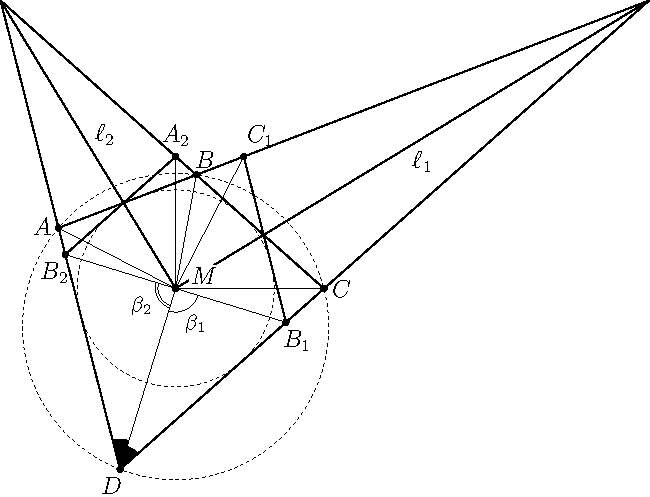
\includegraphics[height=11cm]{./figure.pdf}
\end{figure}


Пусть прямая \(\ell_1\) --- ГМТ точек, равноудалённых от прямых \(AB\) 
и \(CD\), а прямая \(\ell_2\) --- ГМТ точек, равноудалённых от прямых 
\(BC\) и \(AD\), причём \(\ell_1 \cap \ell_2 = M\). 
%Сделаем симметрию относительно прямой \(\ell_1\). 
%Ясно, что прямая \(AB\) перейдёт в 
%прямую \(CD\) и наоборот. 
Точки, симметричные \(B\) и \(C\) относительно \(\ell_1\), обозначим через 
\(B_1\) и \(C_1\) соответственно. Ясно, что они попадут на прямые \(CD\) 
и \(AB\) соответственно. 
Точки, симметричные \(B\) и \(A\) относительно \(\ell_2\), обозначим через 
\(B_2\) и \(A_2\) соответственно. Ясно, что они попадут на прямые \(AD\) 
и \(BC\) соответственно.  


Очевидно, что \(S_{ABCD} = 
S_{AC_1B_1D}\) (\(\triangle BC_1B_1 = \triangle B_1CB\)). 
%Аналогично \(S_{ABCD} = S_{A_2B_2CD}\). 
Из равенства треугольников \(AMB_2\) и 
\(A_2MB\) следует, что 
\(S_{B_2MD} + S_{A_2MC} = S_{AMD} + S_{MBC}
 = S_{AMD} + S_{MB_1C_1}\). 

Пусть теперь 
\(\angle DMB_1 = \beta_1\),
\(\angle DMB_2 = \beta_2\),
\(\angle AMC_1 = \alpha_1\),
\(\angle A_2MC = \alpha_2\).
Тогда \(S_{AC_1B_1D} = S_{DMB_1} + S_{AMC_1} + 
S_{AMD} + S_{MB_1C_1} = S_{DMB_1} + S_{AMC_1} + 
S_{B_2MD} + S_{A_2MC} = 
\bigg(\dfrac{\sin \alpha_1 + \sin \alpha_2}{2}\bigg) 
AM \cdot MC + \bigg(\dfrac{\sin \beta_1 + 
\sin \beta_2}{2}\bigg) BM \cdot MD\).
Из равенств \(S_{AC_1B_1D} = S_{ABCD} = AM \cdot MC + 
BM \cdot MD\), получаем, что  \(\angle \beta_1 = 
\angle \beta_2 = \angle \alpha_1 = \angle \alpha_2 
= 90^{\circ}\). 

Прямоугольные треугольники 
\(DMB_1\) и \(DMB_2\) равны по двум катетам, откуда 
следует, что \(MD\) -- биссектриса угла 
\(\angle ADC\). Следовательно, \(ABCD\) -- описанный, 
ведь точка \(M\) равноудалена от всех его сторон. 
Из того, что \(DM\) является биссектрисой и 
\(\angle DMC = 90^{\circ}\), следует, что 
\(AD \parallel B_1C_1\), что равносильно вписанности 
четырёхугольника \(ABCD\).



%Тогда 
%\(S_{AB_1C_1D} = \)
 
%Очевидно, что если четырёхугольник 
%\(ABCD\) описанный, то и \(



\end{document}
